%statistical analysis
\def\qmutilde{$\widetilde{q_{\mu}}$\xspace}
\def\muhat{$\hat{\mu}$\xspace}
\def\thetahat{$\hat{\theta}$\xspace}
\def\thetahathat{$\hat{\hat{\theta}}$\xspace}
\def\cls{$CL_{s}$\xspace}
\def\clsb{$CL_{s+b}$\xspace}
\def\clb{$CL_{b}$\xspace}

%%\paragraph{}
The statistical techniques used in this search are the same as adopted in: \cite{ATLASHHbbbb} and \cite{ATLAS-CONF-2016-017} and summarized below for completeness.

%%\paragraph{}
Results shown in this section are obtained with the RSG model with c=1.0, RSG with c=2.0 and 2HDM models.

%\subsection{Signal interpolation}
%\label{sec:SigInterpolation}
%%\input{Sections/sec-signal-interpolation}

\subsection{Search procedure}
\label{sec-search-procedure}
% 
% p-value calculation to search for an excess
%
%%\paragraph{}
The statistical analysis of the data after unblinding consists first in a search for statistically significant deviation from the background model hypothesis.  The test statistic used is a one sided profile likelihood ratio \cite{AsymLikelihood}:

\begin{equation}
  {q_{0}} =
  \begin{cases}
    -2ln \frac{L(0,\hat{\hat{\theta}}(0))}{L(\hat{\mu},\hat{\theta})} & \hat{\mu} > 0 \\
    0 & \hat{\mu} < 0
  \end{cases} 
\end{equation}

\noindent
Where, $\mu$ is the value of the signal normalization considered, \muhat is the maximum likelihood (ML)  value of $\mu$. $\theta$ are the set of nuisance parameters (NP), \thetahat is the ML value of $\theta$ and  \thetahathat is the ML value of $\theta$ when $\mu$ is fixed at a particular value. L denotes the profile likelihood, L(\muhat, \thetahat) is the likelihood where $\mu$ is allowed to take any value, the  unconstrained likelihood. L(0, \thetahathat) is the likelihood for the value of $\mu = 0$,  the constrained likelihood.

%%\paragraph{}
This tests the compatibility of the data with the background-only hypothesis, $\mu = 0$. The local p-value of a set of data, $p_0$, is defined as the probability for the background-only hypothesis to have a value of $q_0$ that is as high or higher than the value of $q_{0}$ in that data. In order to obtain $p_0$, pseudo-experiments are generated with the background only model and the distribution of the test statistic, $q_{0}$, is built up from the values of the pseudo-experiments.

%%\paragraph{}
RS graviton signal samples are tested with masses between 300~$<~M_{RSG}~<$~3000 GeV at 100 GeV intervals up to 1600 GeV, with 200 GeV intervals up to 2000 GeV and with 250 GeV intervals between 2000 and 3000 GeV.

%%\paragraph{}
If a local $p_{0}$ value is obtained that corresponds to a significance of greater than $3\sigma$ then a correction for the look elsewhere effect will be computed in order to obtain the global p-value. This correction is obtained using the distribution of the test statistic, $q_{0}$, in background only pseudo-experiments. The average number of upwards crossings, $<N_{1\sigma}>$, across the mass range tested of $q_{0}$ at the value of $q_{0}$ corresponding to $1\sigma$ significance, $q_{0}^{1\sigma}$, is estimated using the average number from the background only pseudo-experiments and is used to obtain the correction to the local p-value using the equation:

\begin{equation}
  p_{0}^{global} = p_{0}^{\text{local}} + <N_{1\sigma}>e^{-(q_{0}^{max} - q_{0}^{1\sigma})/2}
\end{equation}

\noindent
Where $p_{0}^{\text{local}}$ is the lowest $p_{0}$ value across the mass range tested, 
corresponding to a test statistic value of $q_{0}^{max}$. 


\subsection{Limit setting procedure}

% If any significant deviation from the background-only hypothesis (defined as a global p-value 
% corresponding to a significance in excess of 3$\sigma$) is observed then an upper limit on the RSG 
% signal cross-section is going to be derived using the following procedure.

\subsubsection{Choice of exclusion statistics}

%%\paragraph{}
To evaluate an upper limit of $\sigma(\mathrm{G} \to{\mathrm{hh}}\to b\bar{b}b\bar{b})$  a frequentist method is used where a cross section is excluded on the basis of the statistic  \cls~\cite{Read:2002hq}, which is defined as the ratio of \clsb to \clb. Where \clsb is defined as $P_{s+b}(q \le q_{obs})$, i.e. the probability of the signal+background  model to produce data with a value of q less than that observed. Where q is a test statistic, which tests the compatibility with the signal+background hypothesis, where low values indicate a high level of compatibility. \clb = $P_{b}(q \le q_{obs})$, i.e. the probability of the background model to produce data with the same or more compatibility with the signal+background model as that observed. Cross sections are excluded if they have a value of \cls $\le 0.05$.  

%%\paragraph{}
In order to calculate the p-values used to determine \clsb and \clb, the test statistic chosen is a one-sided profile likelihood ratio defined as:

\begin{equation}
  \widetilde{q_{\mu}} =
  \begin{cases}
    -2ln \frac{L(\mu,\hat{\hat{\theta}}(\mu))}{L(0,\hat{\hat{\theta}}(0))} & \hat{\mu} < 0 \\
    -2ln \frac{L(\mu,\hat{\hat{\theta}}(\mu))}{L(\hat{\mu},\hat{\theta})} & 0 \le \hat{\mu} < \mu \\
    0 & \hat{\mu} > \mu
  \end{cases} 
\end{equation}

\noindent 
Where, $\mu$ is the value of the signal normalization considered, \muhat is the maximum likelihood (ML) value of $\mu$. $\theta$ are the set of nuisance parameters, \thetahat is the ML value of $\theta$ and \thetahathat is the ML value of $\theta$ when $\mu$ is fixed at a particular value. L denotes the profile likelihood, L(\muhat, \thetahat) is the likelihood where $\mu$ is allowed to take any value, the unconstrained likelihood. L($\mu$, \thetahathat) is the likelihood for a particular fixed value of $\mu$, the constrained likelihood.

%%\paragraph{}
The definition of the test statistic, \qmutilde, takes into account the fact that when searching 
for a resonance on top of a background the case where $\mu < 0$ is unphysical.

\subsubsection{Calculation of the test statistic}

%%\paragraph{}
In order to obtain the distributions of the test statistic, \qmutilde, two approaches are usually considered: the asymptotic approximation and the toy-MC method.

%%\paragraph{}
In the case of the asymptotic approximation the equations obtained in \cite{AsymLikelihood} are solved numerically. These equations can be derived using approximations  of the distribution of \muhat as Gaussian and the asymptotic approximation of the distribution of the profile likelihood ratio to a non-central chi-squared distribution. 

%%\paragraph{}
The toy MC method works instead by generating datasets randomly sampling the background and signal plus background models, calculating the value of \qmutilde for each individual dataset and then plotting these in a histogram to obtain the distributions and hence the p-values.

%%\paragraph{}
The exclusion limits, for an individual signal mass point, are obtained by scanning over the values of $\mu$, generating 10000 background and 10000 signal+background toys to find the p-values at that $\mu$ point and interpolating to find the value of $\mu$ at which \cls = 0.95. This is done for the data point in the case of the observed limit, for the median value of the background only distribution in the case of the expected limit and for the points which contain 68\%/95\% of the background only distribution in the case of the $\pm 1/2\sigma$ bands on the expected limits. 

\pagebreak{}
\subsection{Expected Limits with statistical uncertainty only}
\label{sec:expectedlimits_stat}

The expected exclusion limits for the KK graviton model with  $c \equiv k/\bar{M}_P = 1.0$
and including only statistical uncertainty are shown in Figure ~\ref{fig:brazil_hh_boosted_4b_c10_stat}, ~\ref{fig:brazil_hh_boosted_3b_c10_stat}, ~\ref{fig:brazil_hh_boosted_2b_c10_stat}. The combined limit of the three channels is shown in Figure ~\ref{fig:brazil_hh_boosted_all_c10_stat}. A comparison to the previous analysis of the 2016 dataset is shown in Figure \ref{fig:Limits_2017_ICHEP_StatOnly}.

\begin{figure*}
\begin{center}
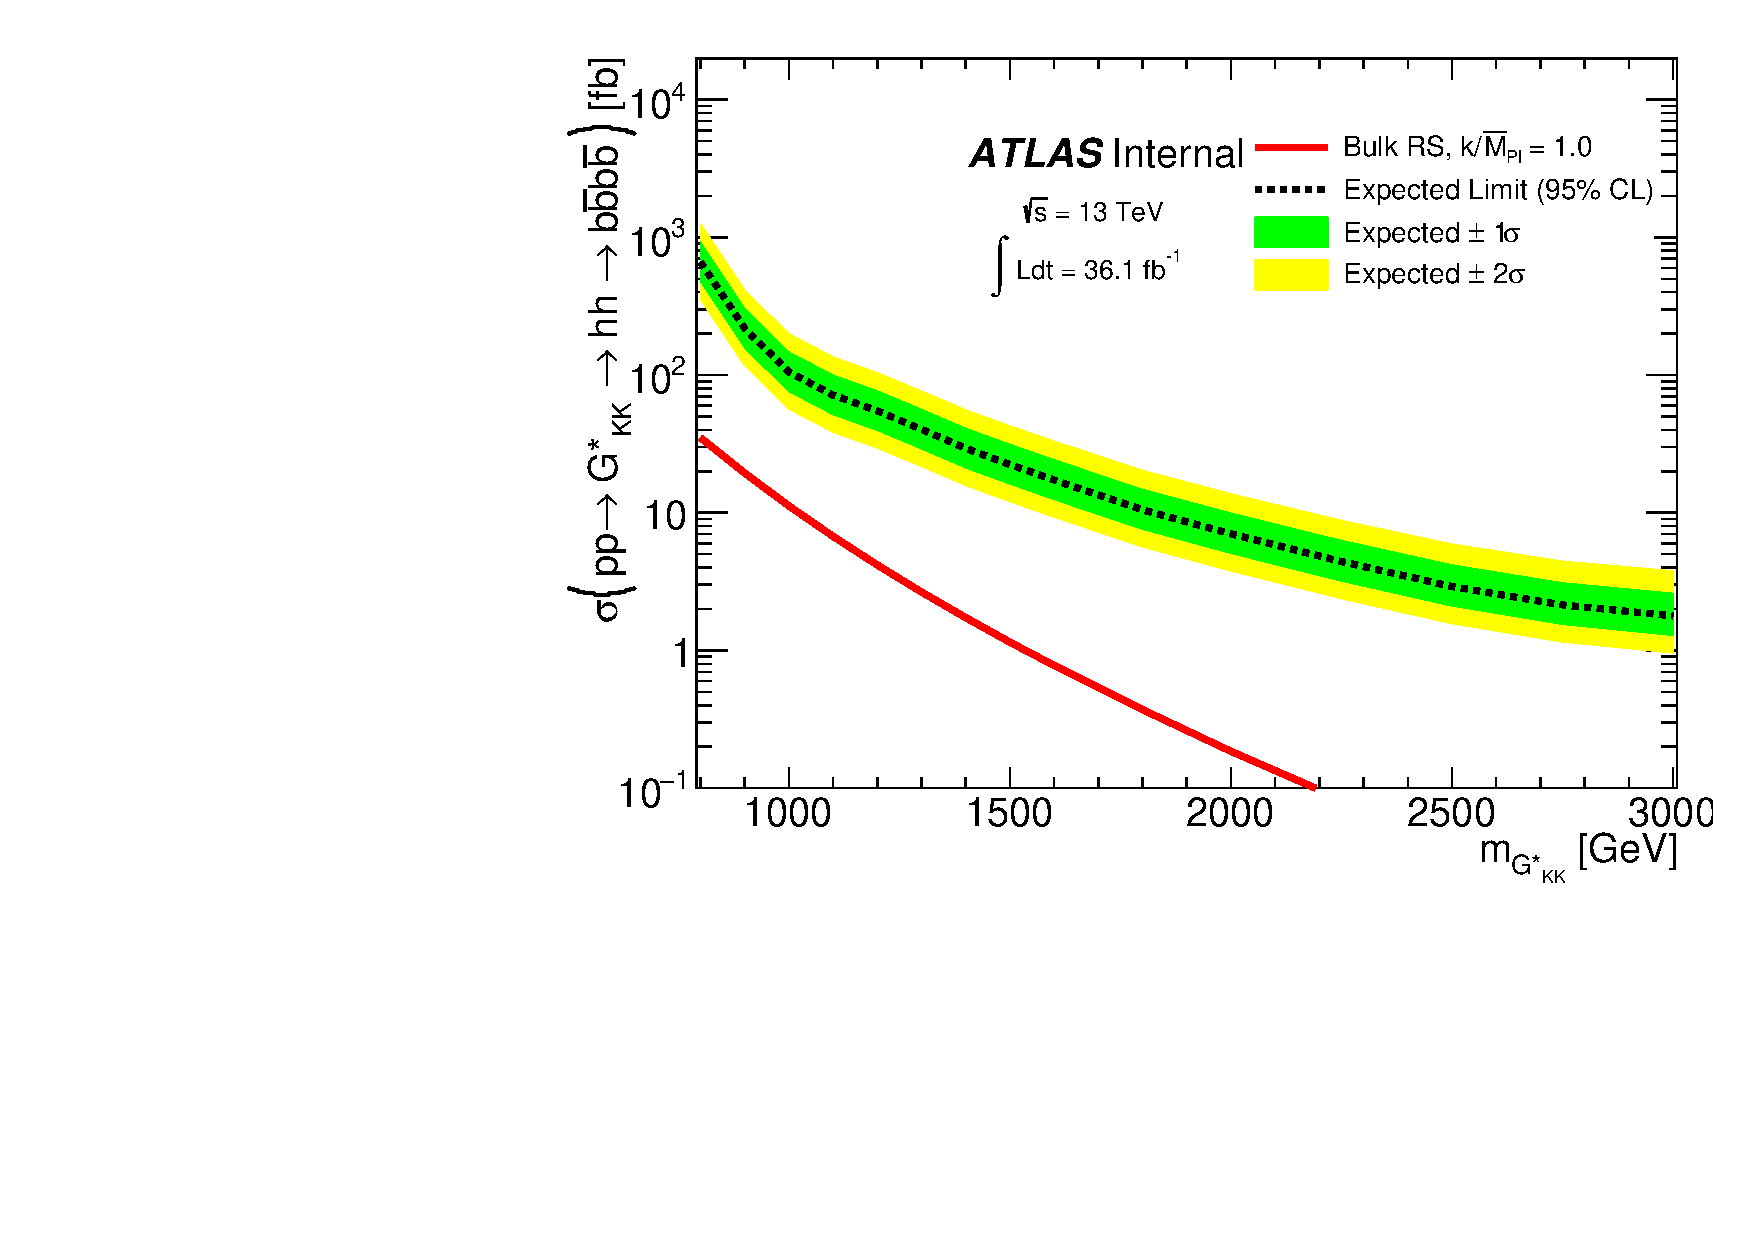
\includegraphics[width=0.78\textwidth,angle=-90]{figures/boosted/Limit_Stat/BrazilPlot_Asymptotic_RSGC10_merged_2b.pdf}
\caption{The expected exclusion limits for the boosted $4b$ analysis calculated including statistical uncertainty only
for the KK graviton model with $c \equiv k/\bar{M}_P = 1.0$. Limits are derived within the asymptotic approximation.}
\label{fig:brazil_hh_boosted_4b_c10_stat}
\end{center}
\end{figure*}

\begin{figure*}
\begin{center}
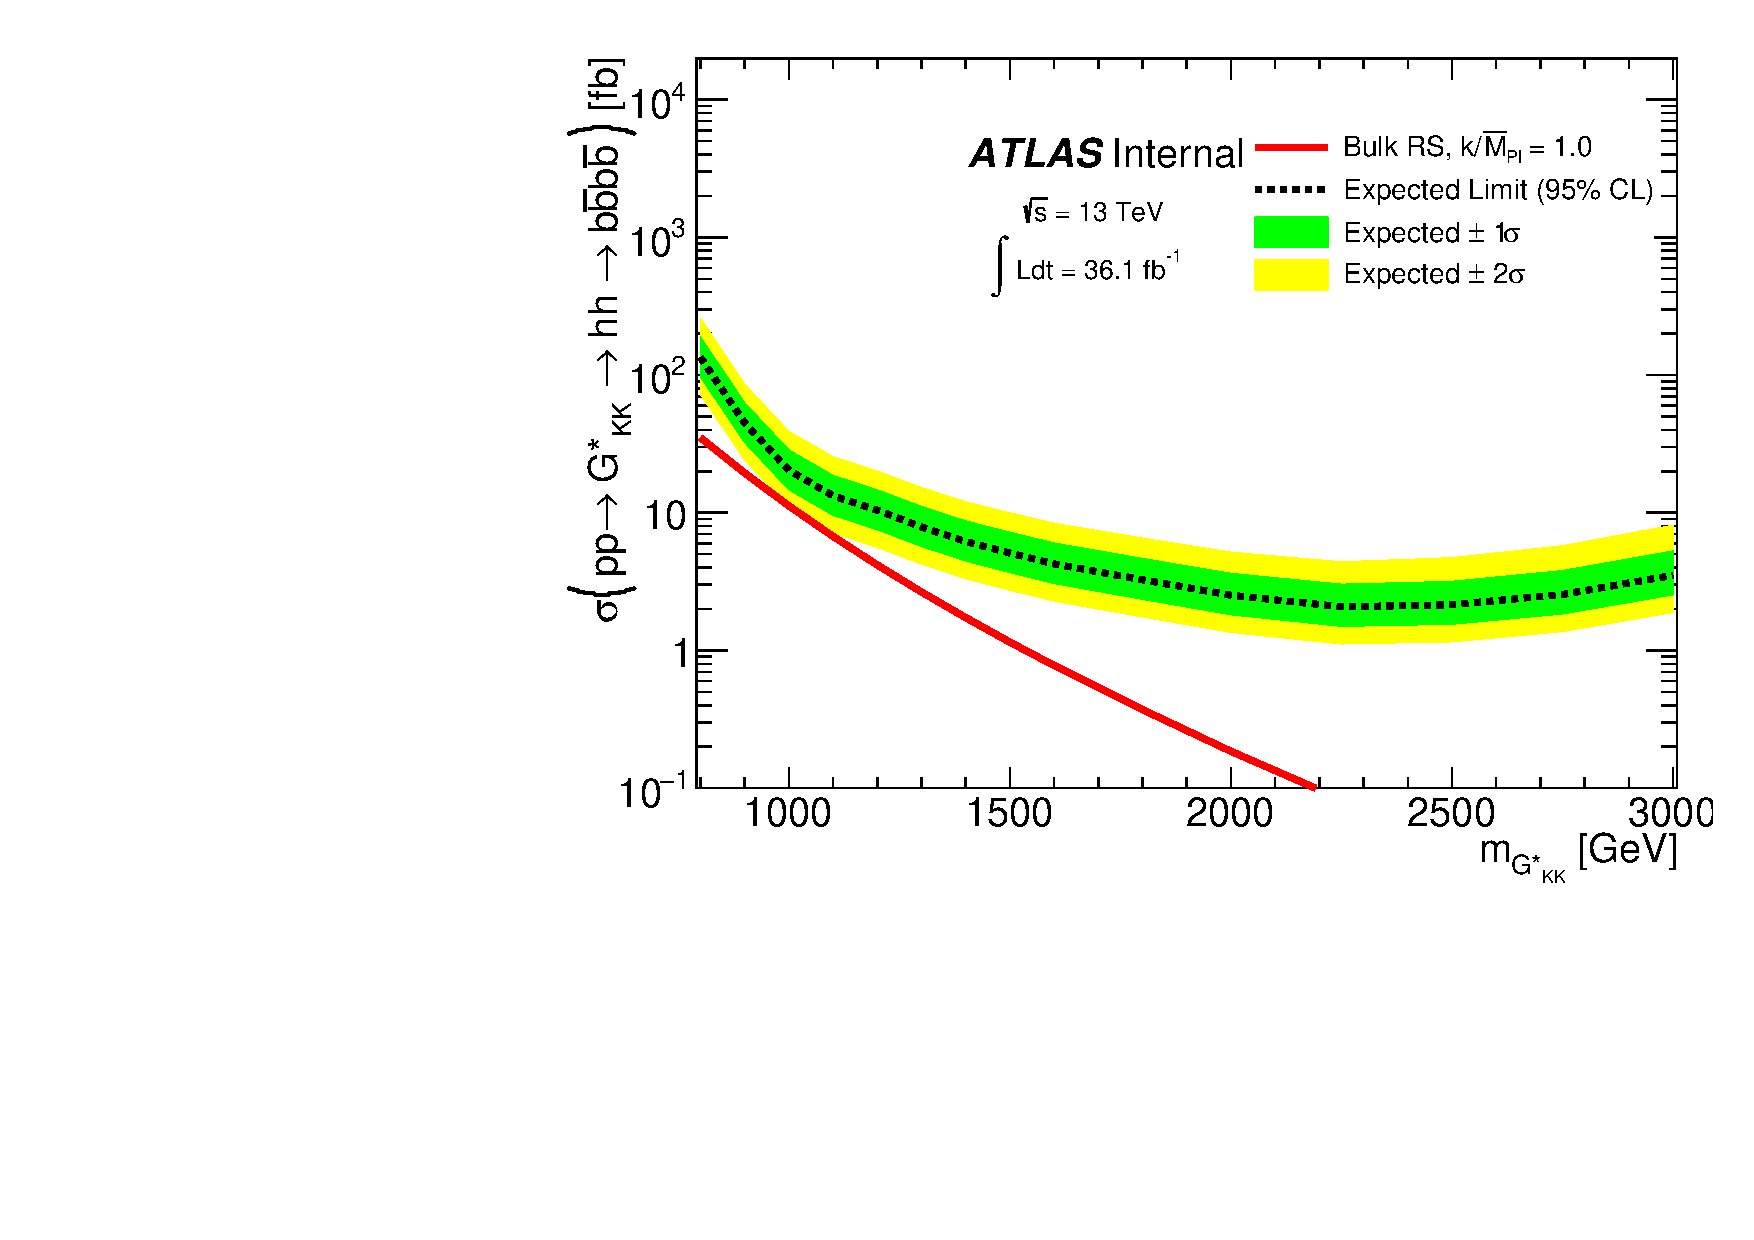
\includegraphics[width=0.78\textwidth,angle=-90]{figures/boosted/Limit_Stat/BrazilPlot_Asymptotic_RSGC10_merged_3b.pdf}
\caption{The expected exclusion limits for the boosted $3b$ analysis calculated including statistical uncertainty only
for the KK graviton model with $c \equiv k/\bar{M}_P = 1.0$. Limits are derived within the asymptotic approximation.}
\label{fig:brazil_hh_boosted_3b_c10_stat}
\end{center}
\end{figure*}

\begin{figure*}
\begin{center}
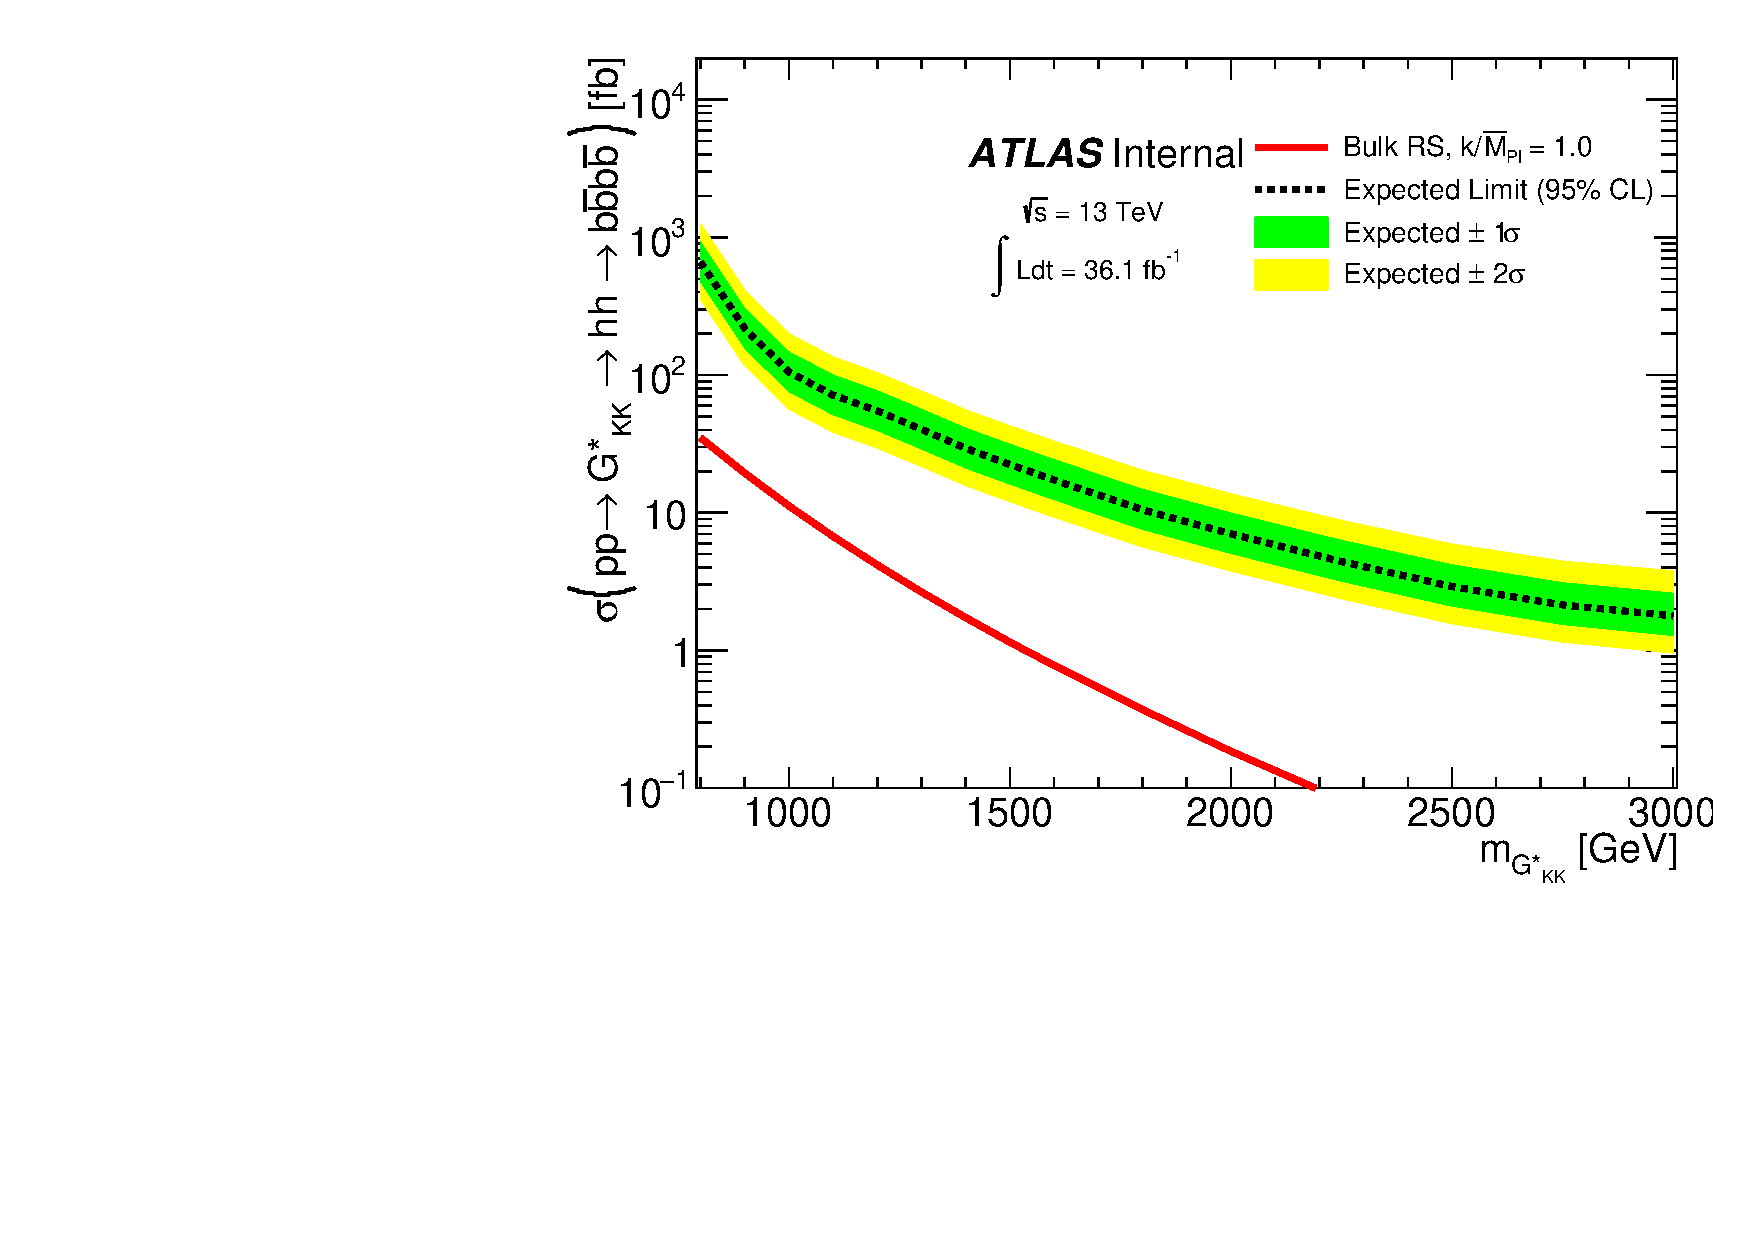
\includegraphics[width=0.78\textwidth,angle=-90]{figures/boosted/Limit_Stat/BrazilPlot_Asymptotic_RSGC10_merged_2b.pdf}
\caption{The expected exclusion limits for the boosted $2bs$ analysis calculated including statistical uncertainty only
for the KK graviton model with $c \equiv k/\bar{M}_P = 1.0$. Limits are derived within the asymptotic approximation.}
\label{fig:brazil_hh_boosted_2b_c10_stat}
\end{center}
\end{figure*}


\begin{figure*}
\begin{center}
%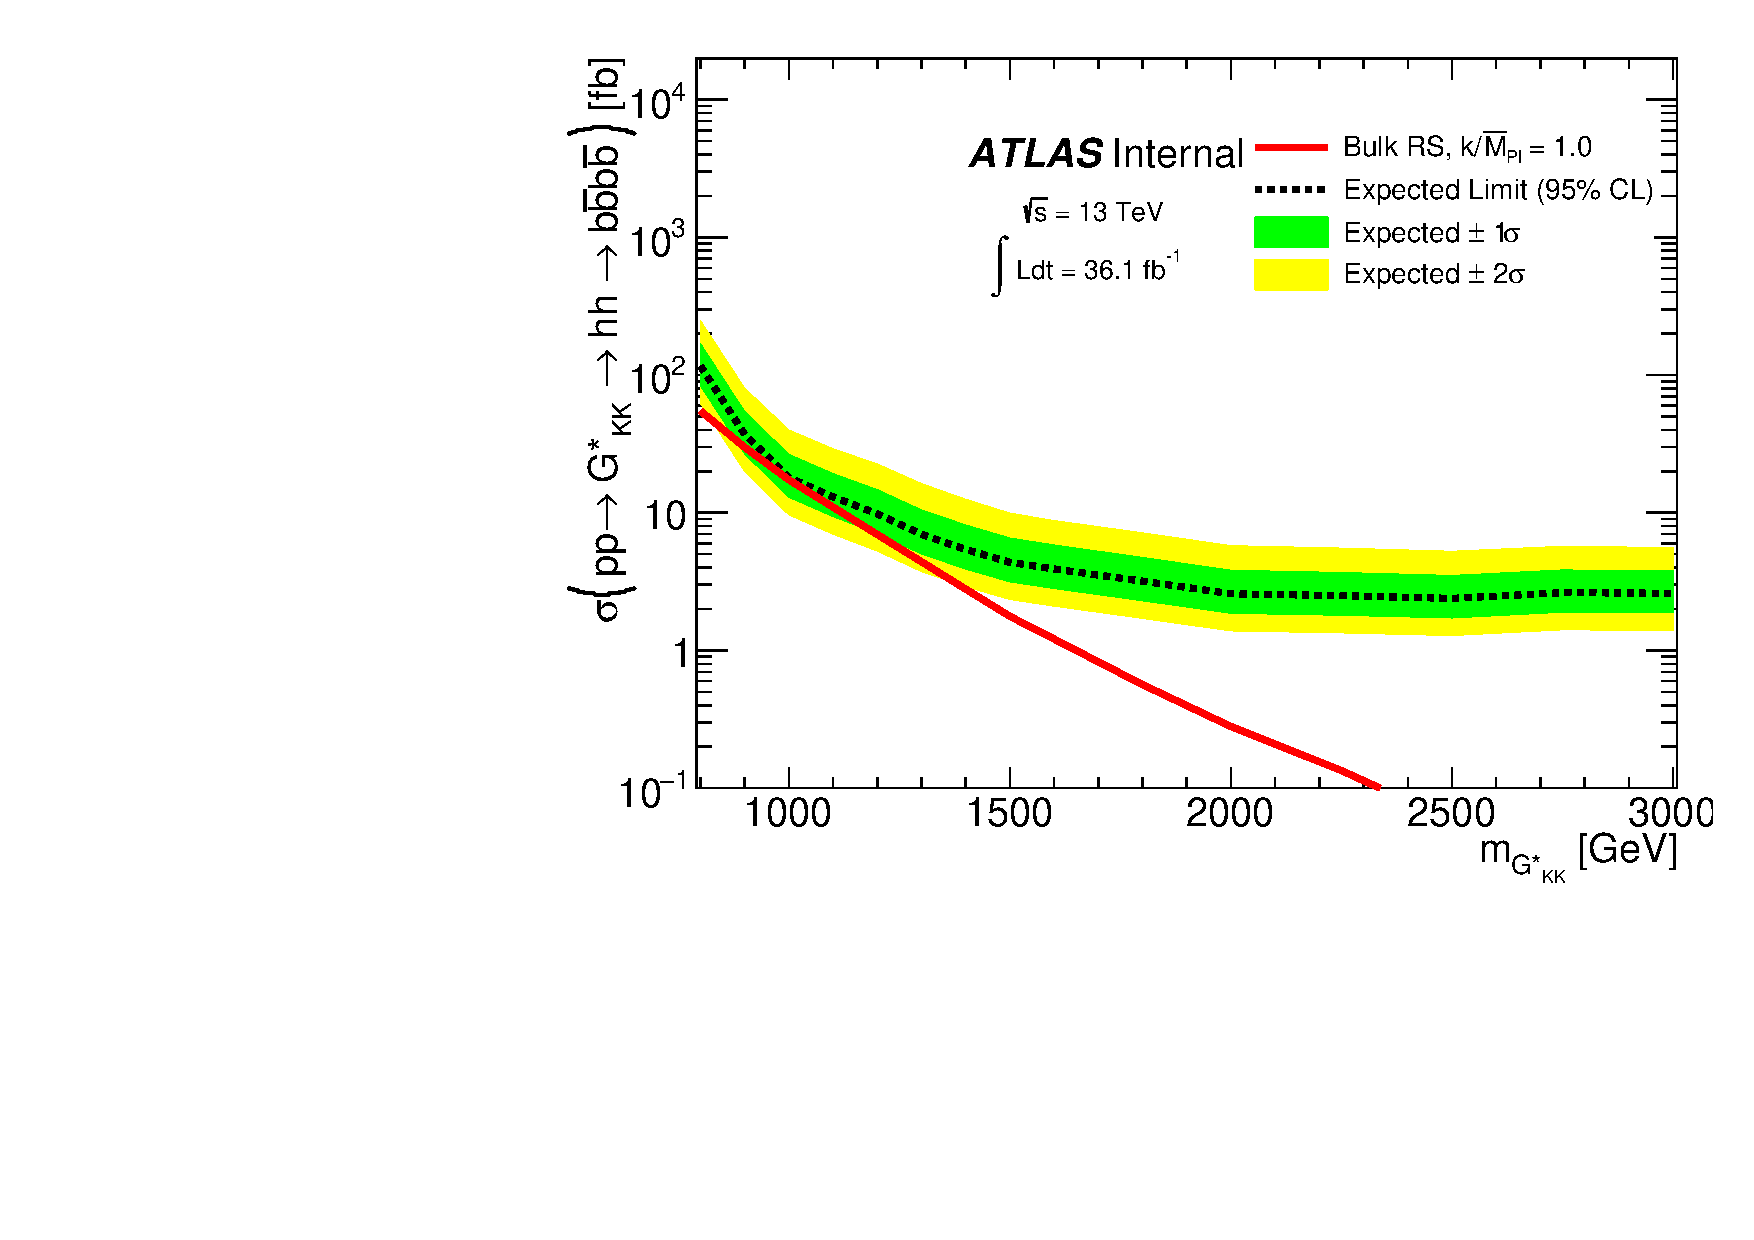
\includegraphics[width=0.78\textwidth,angle=-90]{figures/boosted/Limit_Stat/BrazilPlot_Asymptotic_RSGC10_merged.pdf}
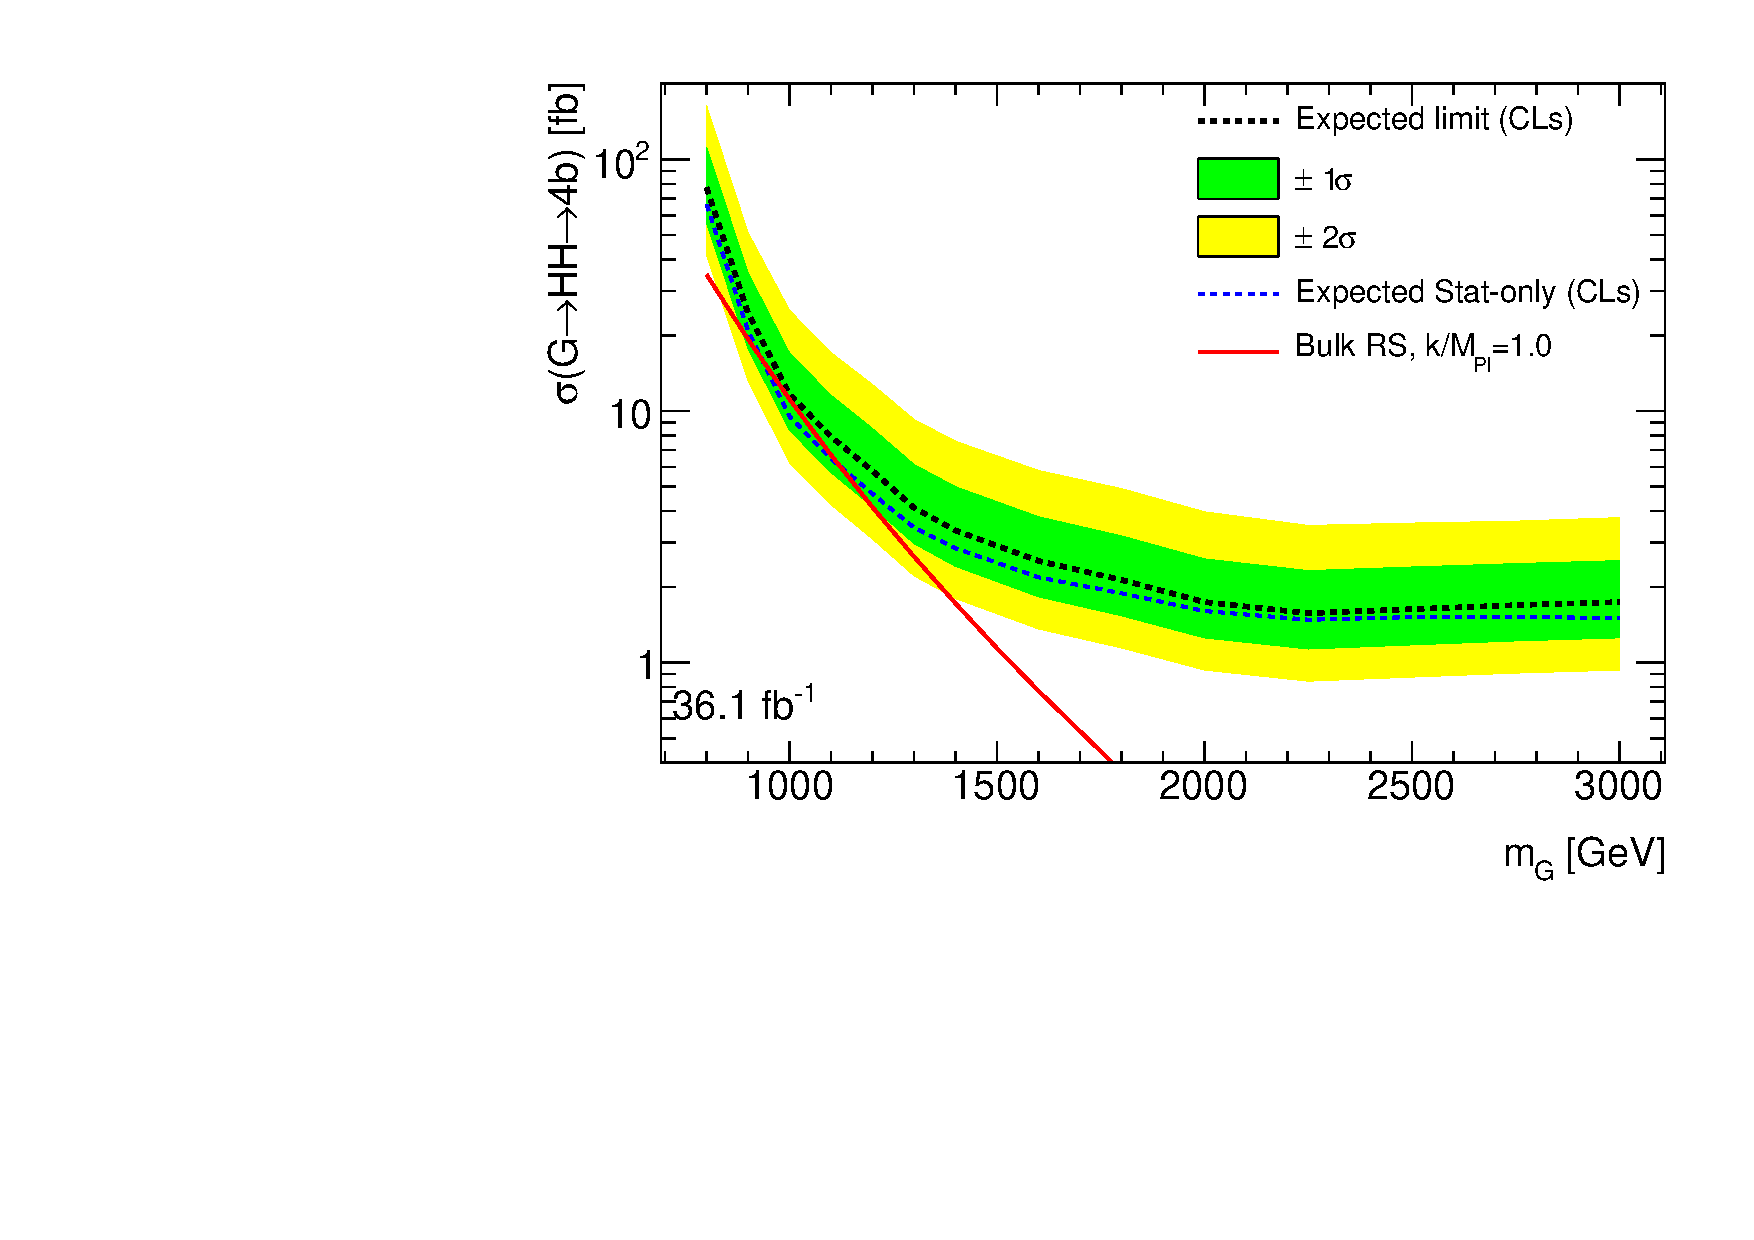
\includegraphics[width=0.78\textwidth,angle=-90]{figures/boosted/Limit_Stat/limit_combined_RSG10_june29.pdf}
\caption{The expected exclusion limits for the combined boosted analysis calculated including statistical uncertainty only and the statistical plus systematic unvertainties for the KK graviton model with $c \equiv k/\bar{M}_P = 1.0$. Limits are derived within the asymptotic approximation.}
\label{fig:brazil_hh_boosted_all_c10_stat}
\end{center}
\end{figure*}

\begin{figure*}
\begin{center}
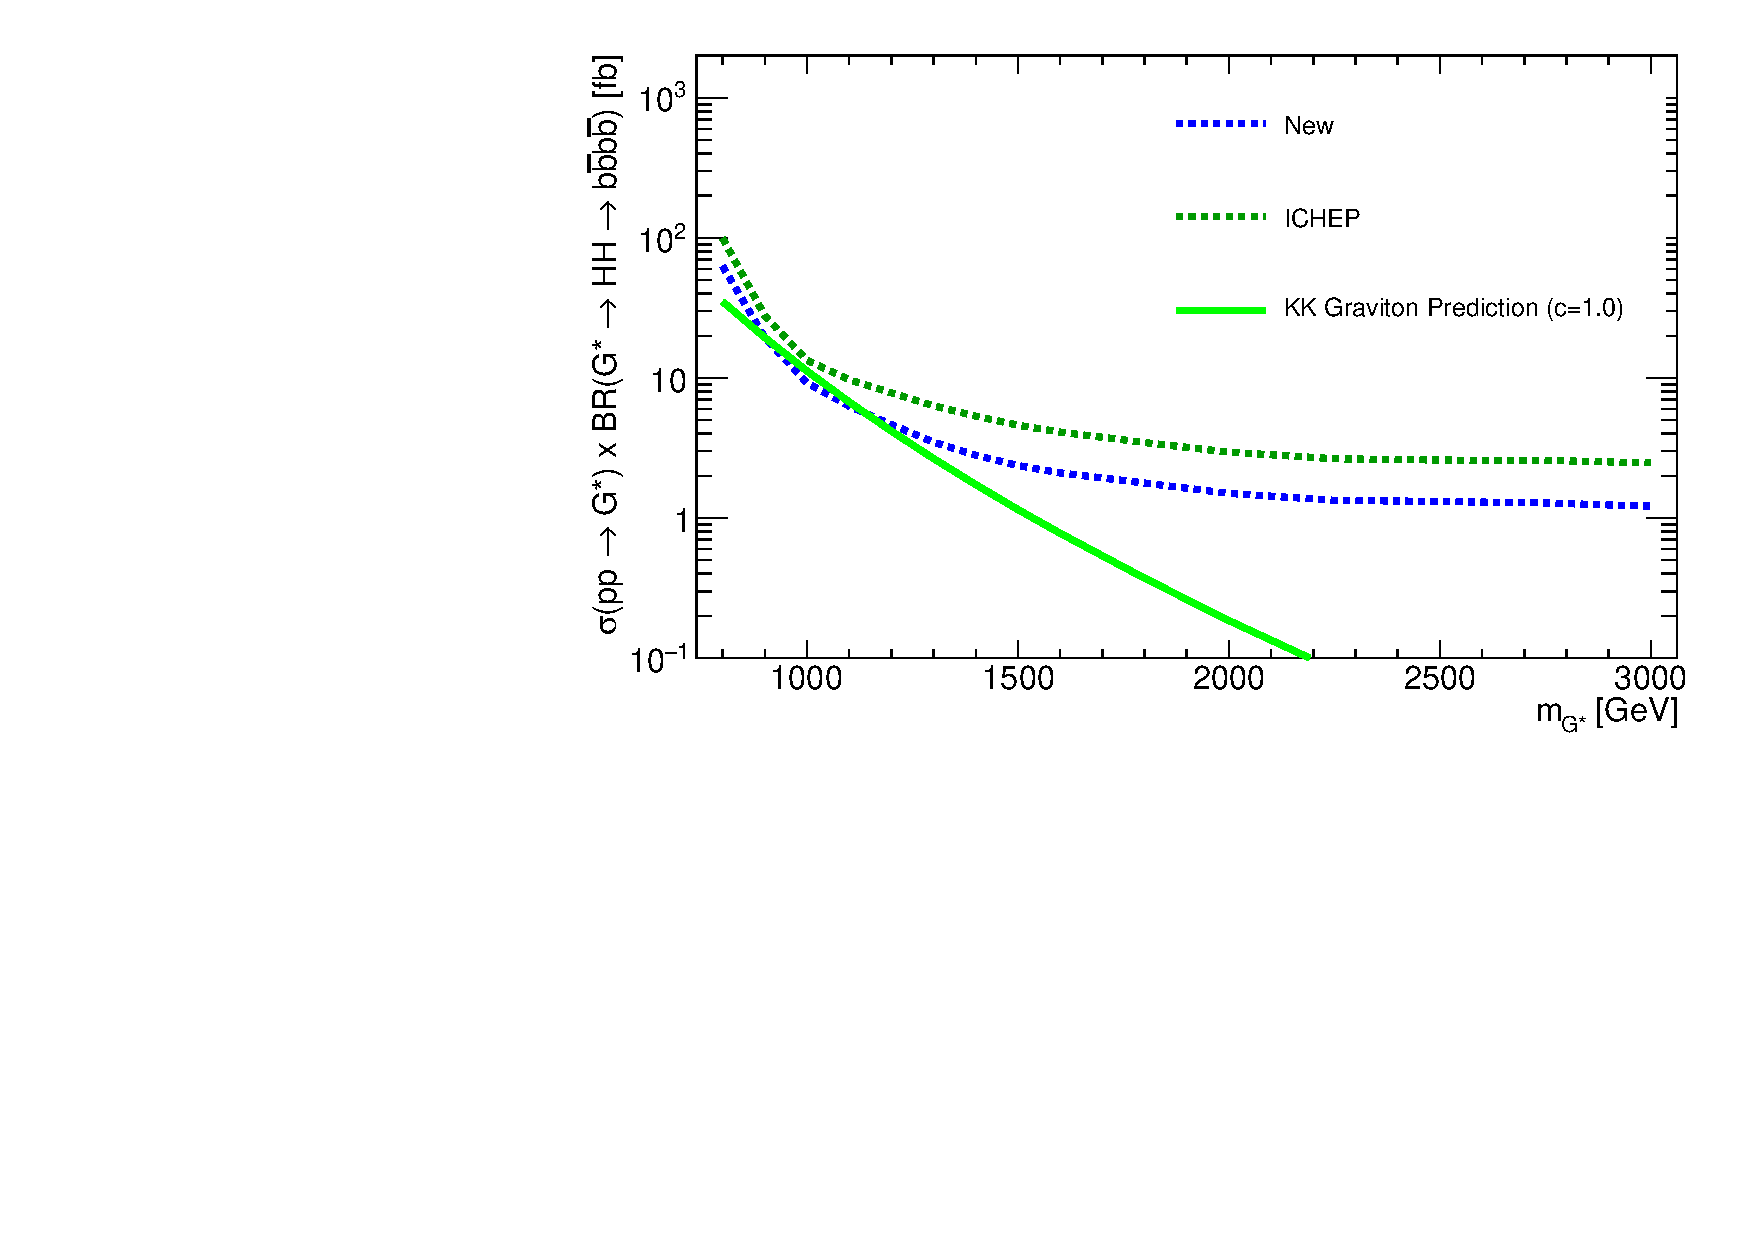
\includegraphics[width=0.78\textwidth,angle=-90]{figures/boosted/Limit_Stat/CompareLimits_HH_Boosted_full2016-ICHEP_c10_ratio.pdf}
\caption{Comparison of 95\% C.L. cross-section limits set in the previous 2015 analysis \cite{ATLAS-CONF-2016-017} to those in the current analysis. Limits are calculated considering only statistical uncertainties for the KK graviton model with $c \equiv k/\bar{M}_P = 1.0$, within the asymptotic approximation.}
\label{fig:Limits_2017_ICHEP_StatOnly}
\end{center}
\end{figure*}
\clearpage


\subsection{Treatment of systematic uncertainties}
\label{sec:limit_sys}


%%\paragraph{}
The following systematic uncertainties will be considered in the final limit calculation:
\begin{itemize}
  \item luminosity uncertainty ($\pm$5\%);
  \item b-tagging scale factor uncertainties;
  \item \largeR jet energy resolution uncertainty;
  \item \largeR jet energy scale uncertainty; 
  \item \largeR jet mass resolution uncertainty;
  \item \largeR jet mass scale uncertainty;
  \item QCD and \ttbar\ normalization uncertainties;
  \item QCD and \ttbar\ shape uncertainties;
  %\item Trigger efficiency uncertainty (resolved analysis only).
\end{itemize}

%%\paragraph{}
They are discussed in sec.~\ref{sec:systematics}. The systematics are treated as constraint terms in the profile likelihood. The default RooStats HistFactory settings are used, which are Gaussian constraint terms with a linear interpolation between the values of the nominal and $\pm 1 \sigma$ histograms for the shape systematics (not changing the normalization) and an exponential interpolation for the  normalization systematics,  which is equivalent to a log-normal constraint term with a linear interpolation between the values. Each uncertainties which impacts both shape and normalization is treated with different constraints as explained above, keeping their variation fully correlated with a single nuisance parameter.


%%\paragraph{}
The asymptotic limits with full systematics for RSG model with c=1.0, RSG with c=2.0 and 2HDM models are shown in Figure ~\ref{fig:brazil_hh_boosted_all_c10_syst}, ~\ref{fig:brazil_hh_boosted_all_c20_syst}, and ~\ref{fig:brazil_hh_boosted_all_2HDM_syst}.

\begin{figure*}
\begin{center}
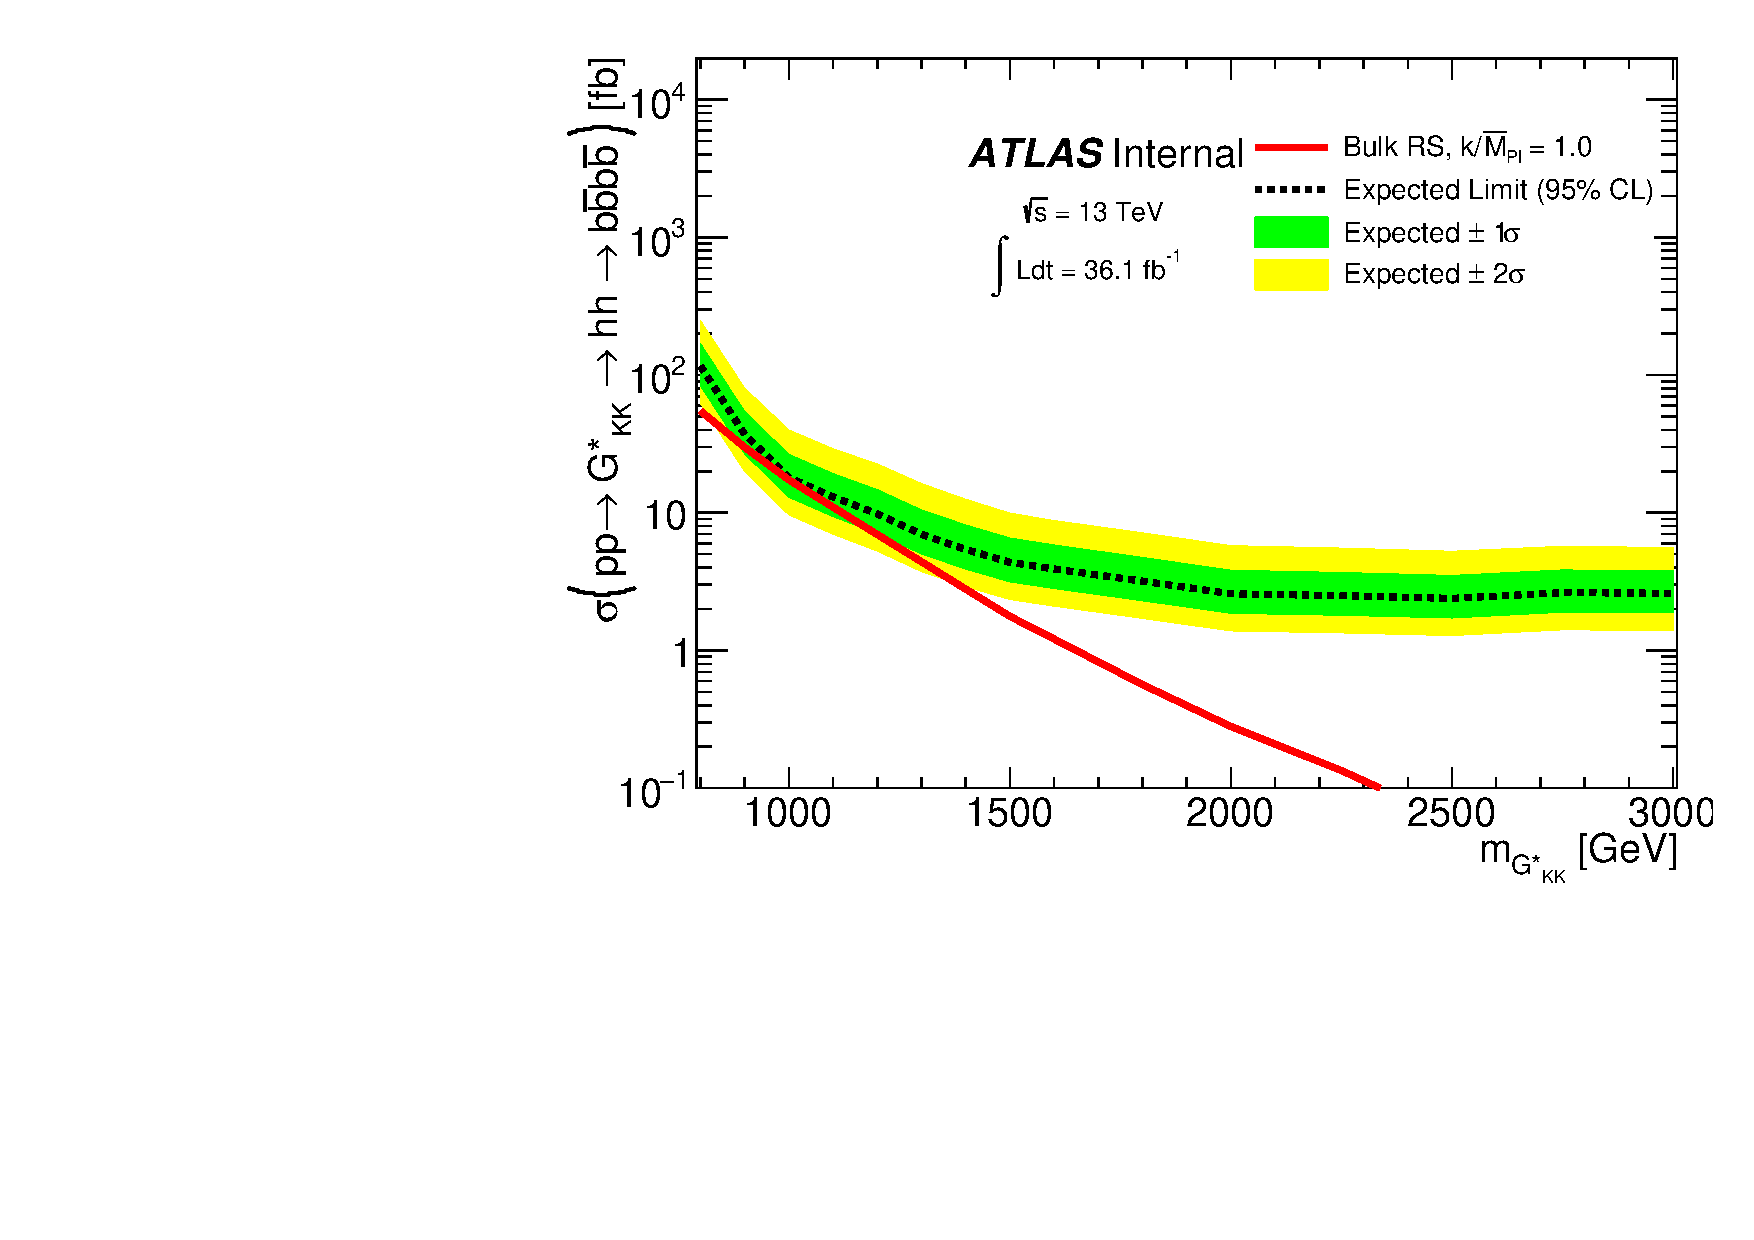
\includegraphics[width=0.7\textwidth,angle=-90]{figures/boosted/Limit_Stat/BrazilPlot_Asymptotic_RSGC10_merged.pdf}
\caption{The expected exclusion limits for the combined boosted analysis calculated including statistical and systematic uncertainty for the KK graviton model with $c \equiv k/\bar{M}_P = 1.0$. Limits are derived within the asymptotic approximation.}
\label{fig:brazil_hh_boosted_all_c10_syst}
\end{center}
\end{figure*}

\begin{figure*}
\begin{center}
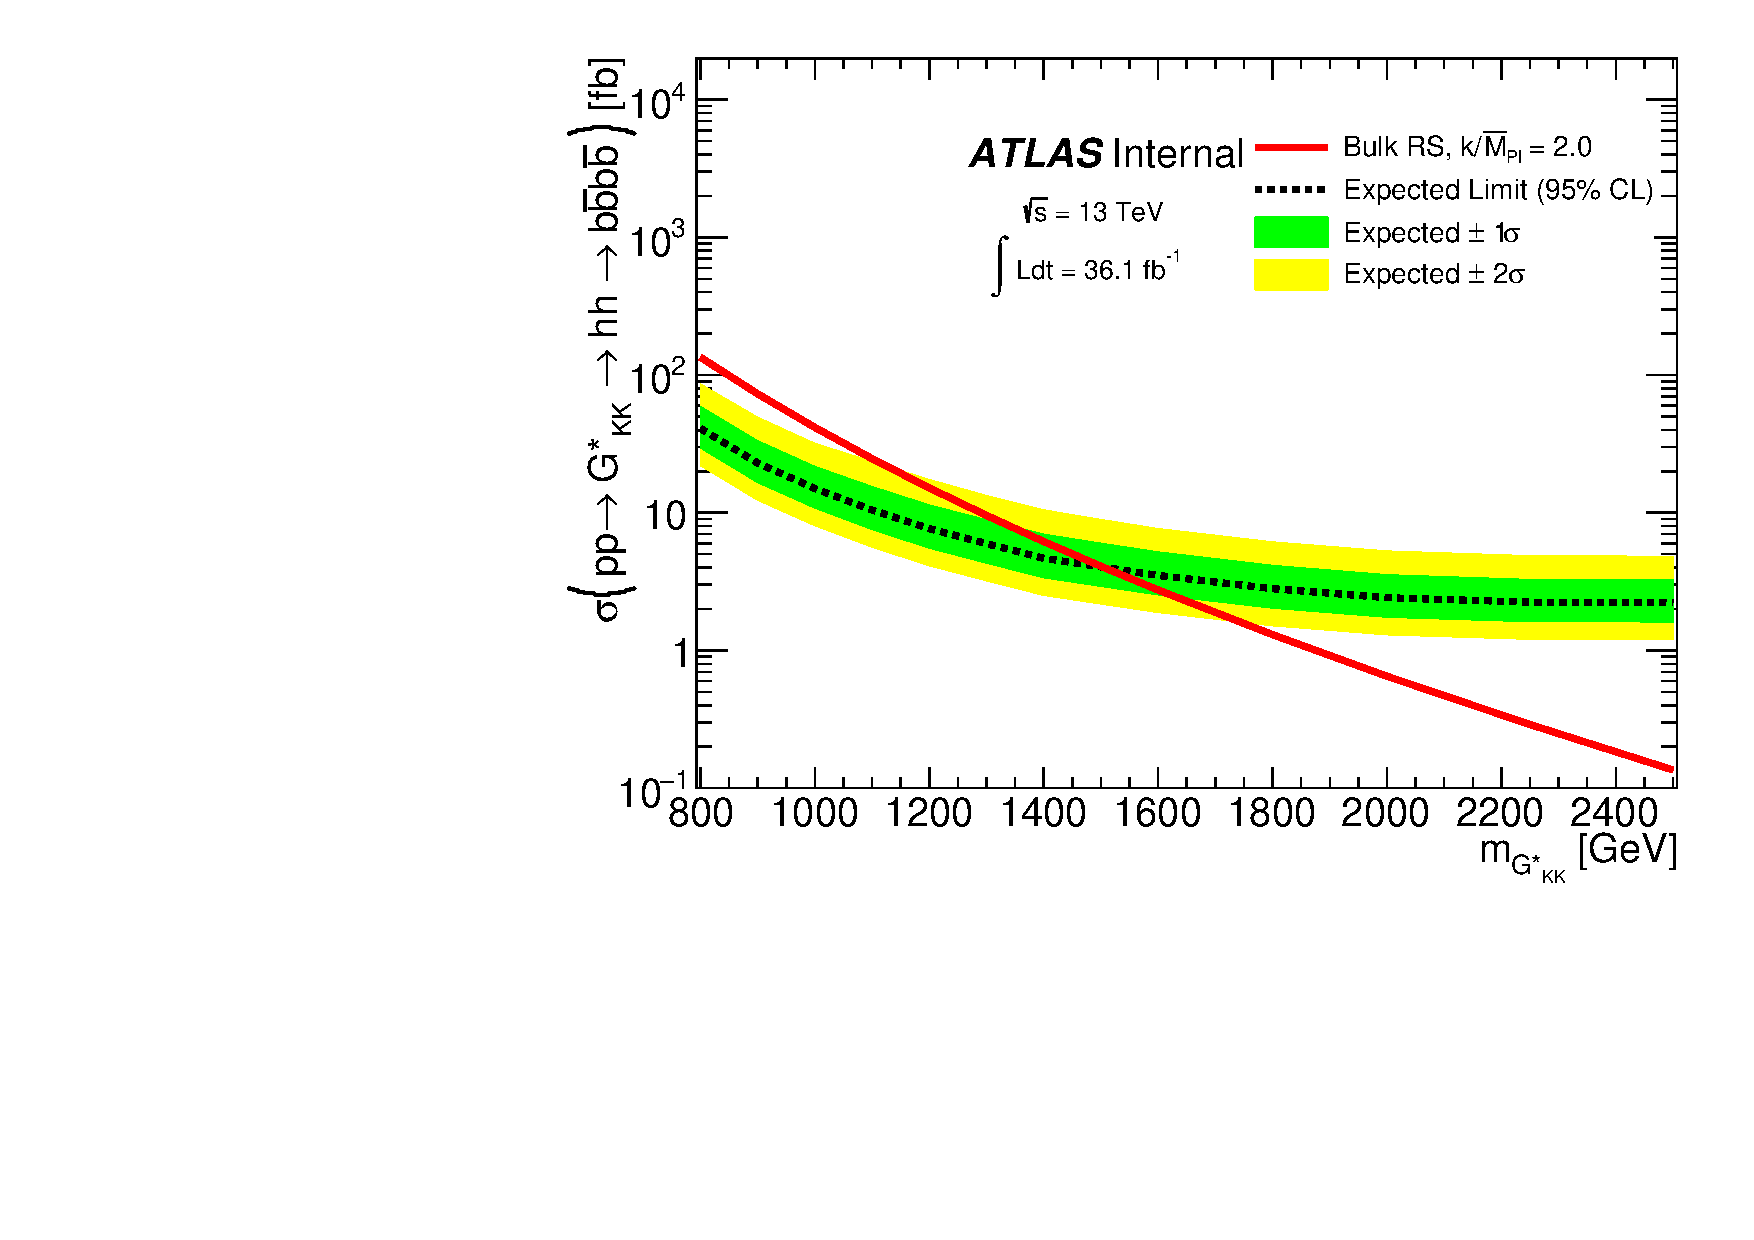
\includegraphics[width=0.7\textwidth,angle=-90]{figures/boosted/Limit_Stat/BrazilPlot_Asymptotic_RSGC20_merged.pdf}
\caption{The expected exclusion limits for the combined boosted analysis calculated including statistical and systematic uncertainty for the KK graviton model with $c \equiv k/\bar{M}_P = 2.0$. Limits are derived within the asymptotic approximation.}
\label{fig:brazil_hh_boosted_all_c20_syst}
\end{center}
\end{figure*}

\begin{figure*}
\begin{center}
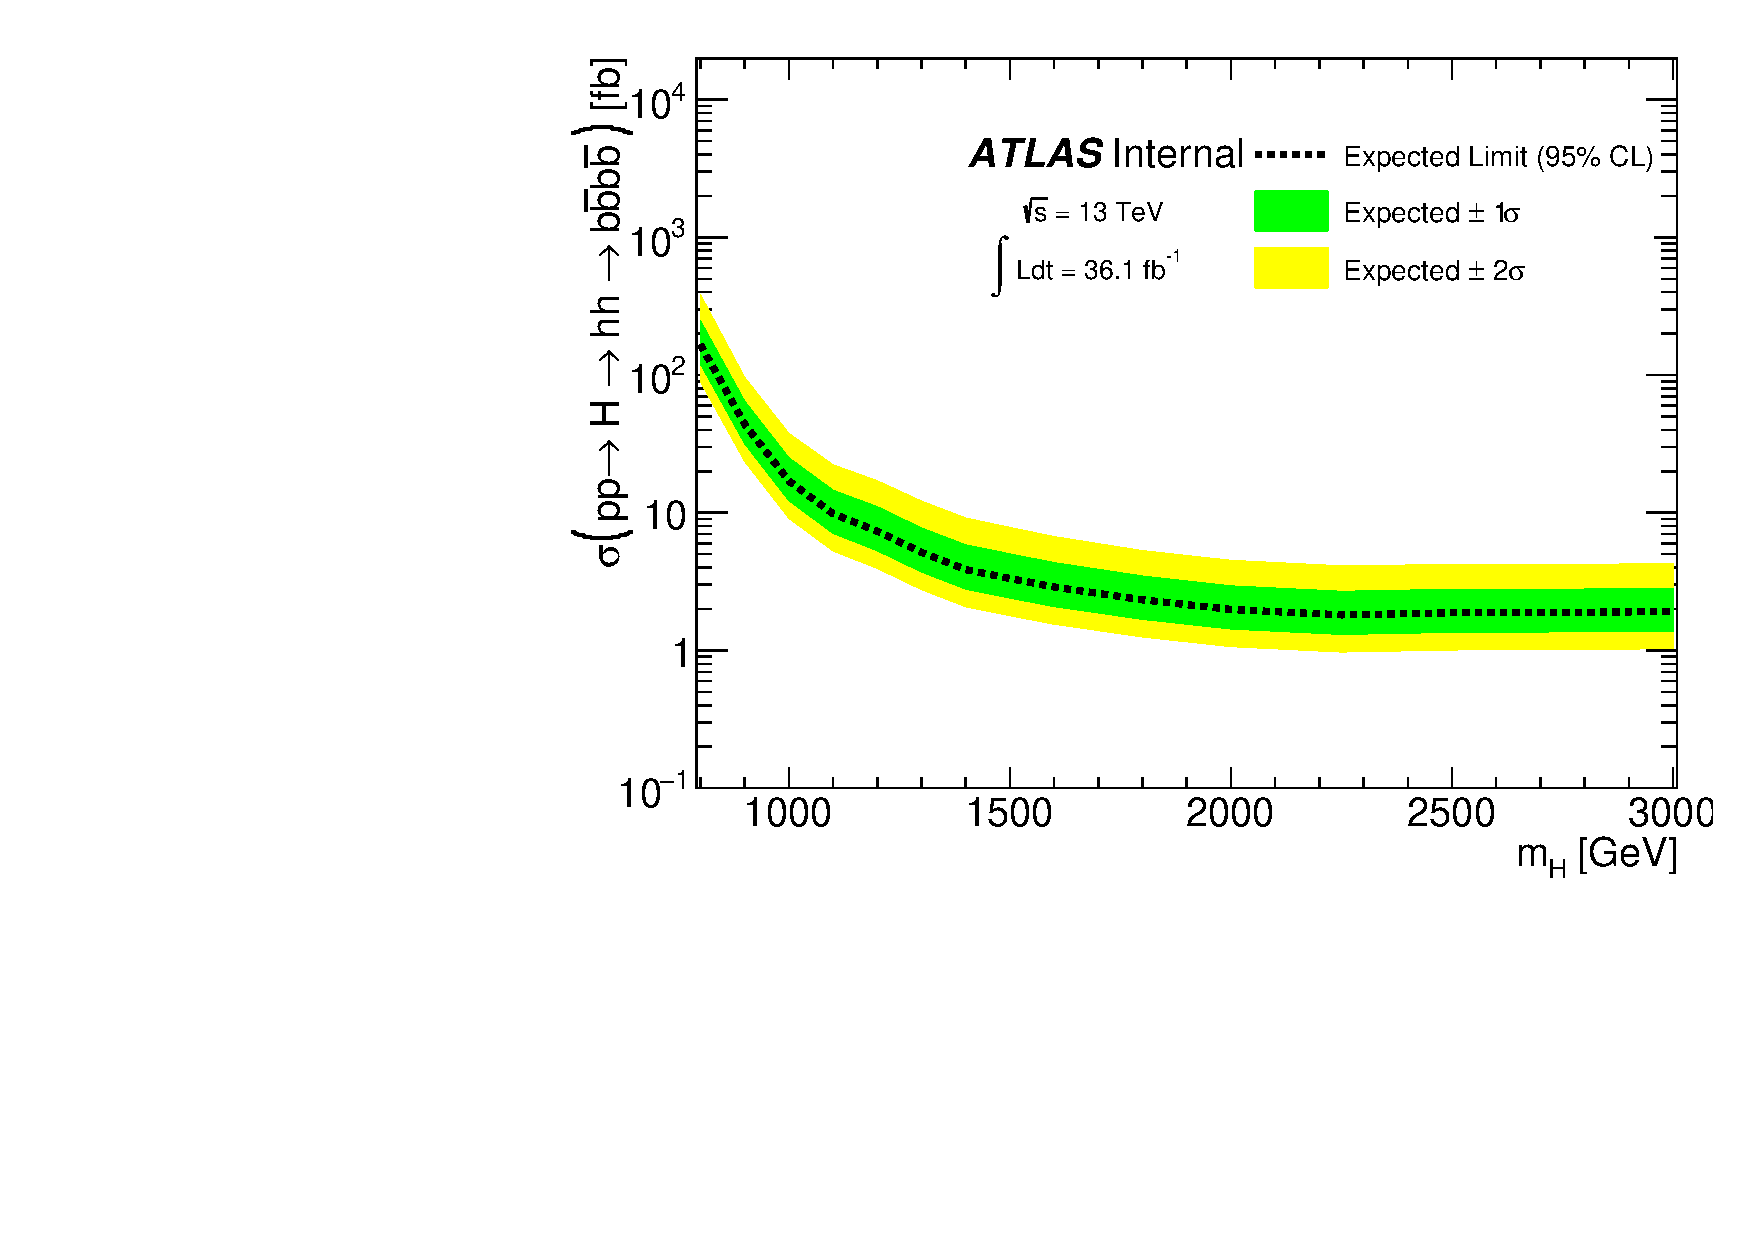
\includegraphics[width=0.7\textwidth,angle=-90]{figures/boosted/Limit_Stat/BrazilPlot_Asymptotic_2HDM_merged.pdf}
\caption{The expected exclusion limits for the combined boosted analysis calculated including statistical and systematic uncertainty for the 2HDM model's heavey Higgs. Limits are derived within the asymptotic approximation.}
\label{fig:brazil_hh_boosted_all_2HDM_syst}
\end{center}
\end{figure*}
% \subsubsection{Impact on the expected limit}
% \begin{figure*}
% \begin{center}
% %%\includegraphics[width=0.45\textwidth]{{figures/StatAnalysis/limits/asymptotic/blinded/SystComponents_RSGC10_resolved_4b_240216_Impact.pdf}}
% \caption{Impact of the different uncertainty sources on the expected exclusion limit when considering all uncertainties.
% The quantity shown on the y-axis is 1 minus the ratio of the limit obtained with all minus one source to the limit with all systematics,
% in percent.
% The signal is the KK graviton model with $c \equiv k/\bar{M}_P = 1.0$. 
% The limits are derived within the asymptotic approximation. TO BE UPDATED.}
% \label{fig:systRanking}
% \end{center}
% \end{figure*}


% \subsubsection{Statistical analysis details}

% Detailed results on the statistical analysis will be reported in this section.
% Pulls of the nuisance parameters (NP) and their correlation matrix will be reported for each mass point
% in Appendix~\ref{app:stat_details_exp}.

% Two type of likelihood fits are considered:
% \begin{itemize}
% \item Unconstrained-likelihood fit: both the NP and the signal strength ($\mu$)
% are fitted to data
% \item Background-only constrained-likelihood fit: $\mu$ is fixed to 0 and only the NP are fitted to data
% \end{itemize}

% For all fits NP pulls are found with mean value $\sim 0$ and width $\sim 1$.
% Some constraint is observed only for the background smoothing uncertainty in
% the boosted channels. This uncertainty is quite conservative at high mass and
% therefore expected to be constrained when fitting pseudo-data represented by the
% expected background prediction.

